In this chapter, we discuss the discontinuous Galerkin (DG) discretization in the velocity variable. Our DG discretization uses Lagrange polynomial bases on Gauss nodes in each velocity cell. This DG discretization is applied to the reduced model kinetic equations in one velocity dimension and to the full Boltzmann equation in three velocity dimensions.
%In both cases, this discretization results in the integral of the Boltzmann collision operator is performed in the three velocity dimensions. In a system of hyperbolic non-homogeneous non-linear equations.

The spatial derivatives are discretized using the finite volume (FV) methods and first and second order temporal splittings are used to advance the reduced model equations in time. In our approach, the spatial and temporal steps are chosen to be uniform, $\Delta x$ and $\Delta t$, respectively. In addition, we develop finite difference (FD) methods for the discretization of the model equations. It will be seen that the first order FD methods and FV methods are identical but we get a difference between the second order FD method and the second order FV method. Splitting techniques will be used to separate the system into the homogeneous transport part and an ODE for the collision part. The CLAWPACK software respects this splitting and will be used to advance the solution of the one dimensional model equations. We use CLAWPACK to solve for the heat transfer problem and the normal shock wave problem. Second order accuracy of the FV method will be verified by solving the homogeneous transport equation and by the shock wave experiment.
%%%%%%%%%%%%%%%%%%%%%%%%%%%%%%%%%%%%%%%%%%%%%%%%%%%%%%%%%%%%%%%%%%%%%%%%%%%%%
%%%%%%%%%%%%%%%%%%%%%%%%%%%%%%%%%%%%%%%%%%%%%%%%%%%%%%%%%%%%%%%%%%%%%%%%%%%%%
\section{Discontinuous Galerkin Discretization in Velocity}
Let us consider the most general form of the gas kinetic equations. This form will include the full Boltzmann equation as well as the BGK and ES-BGK models.
%
\begin{equation}
\label{Boltz}
\frac{\partial}{\partial t} f(\vec{x},\vec{u},t) + \vec{u} \cdot \nabla_{\vec{x}} f(\vec{x},\vec{u},t) = \Psi (f(\vec{x},\vec{u},t))
\end{equation}
%
Where $\Psi (f)$ is the source term describing the collision of molecules. Our motivation is to discretize (\ref{Boltz}) in spatial, temporal and velocity directions. Let us describe the DG discretization that we will be using. Although, strictly speaking, the velocity domain is infinite, we can select some finite interval in the $u_1, u_2, u_3$ directions in velocity space sufficiently large enough so that the total amount of gas particles outside of the interval is negligible. Let us define $U := [u_L,u_R] \times [v_L,v_R] \times [w_L,w_R]$ to be such a rectangle. We start by partitioning $U$ into sub rectangles $K_{i,i',i^*} = [u_1^{i-1/2},u_1^{i+1/2}] \times [u_2^{i'-1/2},u_2^{i'+1/2}] \times [u_3^{i^*-1/2},u_3^{i^*+1/2}]$ where $(i,i',i^*) = (1,1,1) \ldots (M,M',M^*)$. Let $\chi_j$ and $\omega_j$ be the nodes and weights of Gaussian quadrature respectively, and define
%
\begin{align*}
%\label{Gausses}
\chi_{i,j}^u &:= \frac{u_1^{i+1/2} + u_1^{i-1/2}}{2} + \chi_j \frac{u_1^{i+1/2} - u_1^{i-1/2}}{2}\\
\chi_{i',j}^v &:= \frac{u_2^{i'+1/2} + u_2^{i'-1/2}}{2} + \chi_j \frac{u_2^{i'+1/2} - u_2^{i'-1/2}}{2}\\
\chi_{i^*,j}^w &:= \frac{u_3^{i^*+1/2} + u_3^{i^*-1/2}}{2} + \chi_j \frac{u_3^{i^*+1/2} - u_3^{i^*-1/2}}{2}.
\end{align*}
%
For the one dimensional derivations, we simply define $K_i = [u_1^{i-1/2}, u_1^{i+1/2}]$ intervals over $U = [u_L, u_R]$ and use the Gaussian nodes defined in the $u_1$ direction.
%%%%%%%%%%%%%%%%%%%%%%%%%%%%%%%%%%%%%%%%%%%%%%%%%%%%%%%%%%%%%%%%%%%%%%%%%%%%%%%
%%%%%%%%%%%%%%%%%%%%%%%%%%%%%%%%%%%%%%%%%%%%%%%%%%%%%%%%%%%%%%%%%%%%%%%%%%%%%%%
\subsection{The Basis Functions and Their Properties}
On each interval $[u_1^{i-1/2},u_1^{i+1/2}]$ we define our basis functions in one dimension in velocity to be
%
\begin{equation}
\label{basis}
\phi_{i,j}(u_1) := \prod_{k=1 \atop k \neq j}^P \frac{u_1-\chi_{i,k}^{u_1}}{\chi_{i,j}^{u_1} - \chi_{i,k}^{u_1}}.
\end{equation}
%
Three dimensional basis is formed by taking a product of one dimensional basis functions, i.e., 
%
\begin{equation}
\Phi^{i,i',i^*}_{j,j',j^*}(\vec{u}) = \phi_{i,j}(u_1) \phi_{i',j'}(u_2) \phi_{i^*,j^*}(u_3).
\end{equation}
%
Notice that with this choice of the basis our DG approximations coincide with the approximations by the Lagrange interpolating polynomial on each velocity cell.  As we will show next this basis is very convenient for the discretization of the kinetic equations. First of all, let us show that the basis functions are orthogonal. Let's begin with an observation that whenever the basis functions are evaluated on any of the nodes $\chi_{i,k}^u$ we have $\phi_{i,j}(\chi_{i,k}^u) = \delta_{j,k}$ where
%
\begin{equation}
\delta_{j,k} = \left\{
\begin{array}{ll}
1, & j=k \\
0, & j \ne k \\
\end{array} \right.
\end{equation}
%
is the Kronecker delta function. Consequently, we can redefine $\phi_{j,k}^i := \phi_{i,j}(\chi_{i,k}^u)$ and the orthogonality properties follow by applying Gaussian quadrature to the following integrals
%
\begin{align*}
\int_{K_{i,i',i^*}} &\Phi^{i,i',i^*}_{a,b,c}(\vec{u}) \Phi^{i,i',i^*}_{a',b',c'}(\vec{u}) d\vec{u}\\
&= \frac{\Delta u_1^i \Delta u_3^{i'} \Delta u_3^{i^*}}{8} \sum_{p,q,r=1}^{P,Q,R} \omega_p^u \omega_q^v \omega_r^w \Phi^{i,i',i^*}_{a,b,c}(\chi_{i,p}^u,\chi_{i',q}^v,\chi_{i^*,r}^w) \Phi^{i,i',i^*}_{a',b',c'}(\chi_{i,p}^{u_1},\chi_{i',q}^{u_2},\chi_{i^*,r}^{u_3})\\
&= \frac{\Delta u_1^i \Delta u_3^{i'} \Delta u_3^{i^*}}{8} \omega_a^u \omega_b^v \omega_c^w \delta_{a,a'} \delta_{b,b'}
\end{align*}
%
and
%
\begin{align*}
&\int_{K_{i,i',i^*}}
\left(
\begin{array}{c}
u \\
v \\
w \\
\end{array} \right)
\Phi^{i,i',i^*}_{a,b,c}(\vec{u}) \Phi^{i,i',i^*}_{a',b',c'}(\vec{u}) d\vec{u}\\
&= \frac{\Delta u_1^i \Delta u_3^{i'} \Delta u_3^{i^*}}{8} \sum_{p,q,r=1}^{P,Q,R} \left(
\begin{array}{c}
\chi_{i,p} \\
\chi_{i',q} \\
\chi_{i^*,r} \\
\end{array}
\right) \omega_p^u \omega_q^v \omega_r^w \Phi^{i,i',i^*}_{a,b,c}(\chi_{i,p}^u,\chi_{i',q}^v,\chi_{i^*,r}^w) \Phi^{i,i',i^*}_{a',b',c'}(\chi_{i,p}^u,\chi_{i',q}^v,\chi_{i^*,r}^w)\\
&= \frac{\Delta u_1^i \Delta u_3^{i'} \Delta u_3^{i^*}}{8} \omega_a^u \omega_b^v \omega_c^w \left(
\begin{array}{c}
\chi_{i,a} \\
\chi_{i',b} \\
\chi_{i^*,c} \\
\end{array}
\right)
\delta_{a,a'} \delta_{b,b'} \delta_{c,c'}.
\end{align*}
%
Because we used Gaussian quadrature on $P$, $Q$ and $R$ nodes, these quadratures are precise on polynomials of degree $2P-1$, $2Q-1$ and $2R-1$. As you can see the quadrature sums collapsed to just nodal values. This is an important advantages of using the Lagrange polynomial basis.
%%%%%%%%%%%%%%%%%%%%%%%%%%%%%%%%%%%%%%%%%%%%%%%%%%%%%%%%%%%%%%%%%%%%%%%%%%%%%%%%%%%%%%%%%%%%%%%%%%%%%
%%%%%%%%%%%%%%%%%%%%%%%%%%%%%%%%%%%%%%%%%%%%%%%%%%%%%%%%%%%%%%%%%%%%%%%%%%%%%%%%%%%%%%%%%%%%%%%%%%%%%
%%%%%%%%%%%%%%%%%%%%%%%%%%%%%%%%%%%%%%%%%%%%%%%%%%%%%%%%%%%%%%%%%%%%%%%%%%%%%%%%%%%%%%%%%%%%%%%%%%%%%
\subsection{Velocity Discretization}
Now that we have introduced the DG basis functions, we will derive the discretization of the distribution function and the kinetic equations. Let $f^{i,i',i^*}_{p,q,r}(\vec{x},t) = f(\vec{x},\chi_{i,p},\chi_{i',q},\chi_{i^*,r},t)$ and on each $K_{i,i^*,i'}$ we seek the solution in the form:
%
\begin{equation}
\label{fapprox}
f(\vec{x},\vec{u},t) \approx \sum_{p,q,r = 1}^{P,Q,R} f^{i,i',i^*}_{p,q,r}(\vec{x},t) \Phi^{i,i',i^*}_{p,q,r} (\vec{u}).
\end{equation}
%
We then proceed to substitute (\ref{fapprox}) into (\ref{Boltz}) to get
%
\begin{align*}
\frac{\partial}{\partial t} \sum_{p,q,r = 1}^{P,Q,R}& f^{i,i',i^*}_{p,q,r}(\vec{x},t) \Phi^{i,i',i^*}_{p,q,r}(\vec{u}) + \vec{u} \cdot \nabla_{\vec{x}} \sum_{p,q,r = 1}^{P,Q,R} f^{i,i',i^*}_{p,q,r}(\vec{x},t) \Phi^{i,i',i^*}_{p,q,r}(\vec{u})\\
&= \Psi \left(\sum_{p,q,r = 1}^{P,Q,R} f^{i,i',i^*}_{p,q,r}(\vec{x},t) \Phi^{i,i',i^*}_{p,q,r}(\vec{u})\right).
\end{align*}
%
We then multiply both sides by our basis function (\ref{basis}) and integrate over $K_{i,i',i^*}$
%
\begin{align*}
&\int_{K_{i,i',i^*}} \frac{\partial}{\partial t} \sum_{p,q,r = 1}^{P,Q,R} f^{i,i',i^*}_{p,q,r}(\vec{x},t) \Phi^{i,i',i^*}_{p,q,r}(\vec{u}) \Phi^{i,i',i^*}_{p',q',r'}(\vec{u}) d\vec{u}\\
&+ \int_{K_{i,i',i^*}} \vec{u} \cdot \nabla_{\vec{x}} \sum_{p,q,r = 1}^{P,Q,R} f^{i,i',i^*}_{p,q,r}(\vec{x},t) \Phi^{i,i',i^*}_{p,q,r}(\vec{u}) \Phi^{i,i',i^*}_{p',q',r'}(\vec{u}) d\vec{u}\\
&= \int_{K_{i,i',i^*}} \Psi \left(\sum_{p,q,r = 1}^{P,Q,R} f^{i,i',i^*}_{p,q,r}(\vec{x},t) \Phi^{i,i',i^*}_{p,q,r}\vec{u})\right) \Phi^{i,i',i^*}_{p',q',r'}(\vec{u}) d\vec{u}.
\end{align*}
%
We can utilize the orthogonality properties of our basis functions we derived earlier. The transport part of the equation above decouples and the summation terms from the integration collapse to the following form:
%
\begin{gather}
\begin{aligned}
\label{discreting}
\frac{\Delta u_1^i \Delta u_3^{i'} \Delta u_3^{i^*}}{8} &\left( \partial t f^{i,i',i^*}_{p,q,r}(\vec{x},t) + (\chi_{i,p}^u,\chi_{i',q}^v,\chi_{i^*,r}^w) \cdot \nabla_{\vec{x}} f^{i,i',i^*}_{p,q,r}(\vec{x},t) \right) \\
&\approx \int_{K_{i,i',i^*}} \Psi \left(\sum_{p,q,r = 1}^{P,Q,R} f^{i,i',i^*}_{p,q,r}(\vec{x},t) \Phi^{i,i',i^*}_{p,q,r}(\vec{u})\right) \Phi^{i,i',i^*}_{p',q',r'}(\vec{u}) d\vec{u}.
\end{aligned}
\end{gather}
%%%%%%%%%%%%%%%%%%%%%%%%%%%%%%%%%%%%%%%%%%%%%%%%%%%%%%%%%%%%%%%%%%%%%%%%%%%%%%%%%%%%%%%%%%%%%%%%%%%%%%%%%%
\subsection{Discretization of the Macro Parameters}
Recall that the Maxwellian distribution is defined by the first three moments of the velocity distribution function. Particularly, the density, average velocity and temperature are quantities that must be computed. Because these parameters are derived from the distribution function, we need to establish the quadrature formulas for the evaluation of macro parameters from the discrete-velocity solution. Let us observe the number density defined by
%
\begin{equation*}
n = \int_{\mathbb{R}^3} f d\vec{u}.
\end{equation*}
%
Applying the quadrature rule to the integral we obtain
%
\begin{align*}
n &\approx \sum_{i,i',i^*=1}^{M,M',M^*} \int_{K_{i,i',i^*}} f d\vec{u}\\
&= \sum_{i,i',i^*=1}^{M,M',M^*} \int_{K_{i,i',i^*}} \sum_{p,q,r=1}^{P,Q,R} f_{p,q,r}^{i,i',i^*} \Phi_{p,q,r}^{i,i',i^*} d\vec{u}\\
&\approx \sum_{i,i',i^*=1}^{M,M',M^*} \frac{\Delta u_1^{i} \Delta u_3^{i'} \Delta u_3^{i^*}}{8} \sum_{p,q,r=1}^{P,Q,R} f_{p,q,r}^{i,i',i^*} \Phi_{p,q,r}^{i,i',i^*} \omega_p \omega_q \omega_r.
\end{align*}
%
In the case of the one dimensional reduction
%
\begin{equation*}
n \approx \sum_{i=1}^M \frac{\Delta u_1^i}{2} \sum_{p=1}^P h_p^i \phi_p^i \omega_p.
\end{equation*}
%
Similarly, by replacing the integral in the expression for the bulk velocity with numerical quadratures, one arrives at
%
\begin{align*}
\bar{u}_j &= \frac{1}{n} \int_{\mathbb{R}^3} u_i f d\vec{u}\\
&\approx \frac{1}{n} \sum_{i,i',i^*=1}^{M,M',M^*} \frac{\Delta u_1^{i} \Delta u_2^{i'} \Delta u_3^{i^*}}{8} \sum_{p,q,r=1}^{P,Q,R} \chi_{p,q,r}^{u_j} f_{p,q,r}^{i,i',i^*} \Phi_{p,q,r}^{i,i',i^*} \omega_p \omega_q \omega_r.
\end{align*}
%
We notice that in the case of one dimensional problems, the components $u_2$ and $u_3$ of the bulk velocity are zero. Therefore, the one dimensional velocity discretized form of the average velocity takes the form
%
\begin{equation*}
\bar{u}_1 \approx \frac{1}{n} \sum_{i=1}^{M} \frac{\Delta u_1^{i}}{2} \sum_{p=1}^{P} \chi_p^{u_1} h_{p}^{i} \phi_{p}^{i} \omega_p.
\end{equation*}
%
Finally, the discrete velocity equation for the temperature takes the form
%
\begin{align*}
T &= \frac{1}{3 n R} \int_{\mathbb{R}^3} ||\vec{u} - \vec{\bar{u}}||^2 f d \vec{u}\\
&\approx \frac{1}{3 n R} \sum_{i,i',i^*=1}^{M,M',M^*} \frac{\Delta u_1^{i,i',i^*} \Delta u_3^{i,i',i^*} \Delta u_3^{i,i',i^*}}{8} \sum_{p,q,r=1}^{P,Q,R} ||\vec{\chi}_{p,q,r}^{\vec{u}} - \vec{\bar{u}}||^2 f_{p,q,r}^{i,i',i^*} \Phi_{p,q,r}^{i,i',i^*} \omega_p \omega_q \omega_r.
\end{align*}
%
and its one dimensional form is
%
\begin{align*}
T &= \frac{1}{3 n R} \int_{\mathbb{R}} ((u_1 - \bar{u}_1)^2 h + 2g) du_1\\
&\approx \frac{1}{3 n R} \sum_{i=1}^M \frac{\Delta u_1^i}{2} \sum_{p=1}^P ((\chi_p^{u_1} - \bar{u}_1)^2 h_{p}^{i} + 2 g_{p}^{i}) \phi_{p}^{i} \omega_p.
\end{align*}
%\text{and}\\
%\label{temperature}
%T &= \frac{1}{3 n R} \int_{\mathbb{R}^3} ||u - \bar{u}||^2 f d\vec{u} \quad &\text{(Temperature)}.
%\end{align}
%%%%%%%%%%%%%%%%%%%%%%%%%%%%%%%%%%%%%%%%%%%%%%%%%%%%%%%%%%%%%%%%%%%%%%%%%%%%%%%%%%%%%%%%%%%%%%%%%%%%%%%%%%
\subsection{Velocity Discretization of the Kinetic Models}
We now seek to evaluate the right hand side of (\ref{discreting}) for the BGK and ES-BGK models. Let $f_0$ represent the distribution of either the local Maxwellian or general Gaussian distribution wherever appropriate. The right hand side of (\ref{Boltz}) takes the form of
%
\begin{equation}
\label{eq662}
\Psi(f(\vec{x},\vec{u},t)) = \nu \left( f_0(\vec{u}) - f(\vec{x},\vec{u},t) \right)
\end{equation}
%
Applying Gaussian quadrature to the integral (\ref{eq662}) we have
%
\begin{align*}
\int_{K_{i,i',i^*}} &\nu \left( f_0(\vec{u}) - f^{i,i',i^*}_{p,q,r}(\vec{x},t)\Phi^{i,i',i^*}_{p,q,r}(\vec{u}) \right) \Phi^{i,i',i^*}_{p',q',r'}(\vec{u}) d\vec{u} \\
&\approx \nu \left( f_0(\chi_{i,p}^u,\chi_{i',q}^v,\chi_{i^*,r}^w) - f^{i,i',i^*}_{p,q,r}(\vec{x},t) \right) \frac{\Delta u_1^i \Delta u_3^{i'} \Delta u_3^{i^*}}{8}
\end{align*}
%
Then the DG discretized form of (\ref{discreting}) in the case of the BGK and ES-BGK, takes the form of
%
\begin{equation}
\label{DG_BGK_ES}
\partial t f^{i,i',i^*}_{p,q,r}(\vec{x},t) + (\chi_{i,p}^u,\chi_{i',q}^v,\chi_{i^*,r}^w) \cdot \nabla_{\vec{x}} f^{i,i',i^*}_{p,q,r}(\vec{x},t)
= \nu \left( f_0(\chi_{p}^{u_1},\chi_{q}^{u_2},\chi_{r}^{u_3}) - f^{i,i',i^*}_{p,q,r}(\vec{x},t) \right).
\end{equation}
%
In this thesis, we intend to implement the one-dimensional kinetic models. Therefore, this same procedure applied to the one dimensional BGK model gives:
%
\begin{align*}
\partial_t h_p^i + \chi_p^{u_1} \partial_x h_p^i &= \nu \left(\frac{n}{\sqrt{2 \pi RT}} \exp \left( - \frac{(\chi_p^{u_1} - \bar{u}_1)^2}{2 R T} \right) - h \right)\\
\partial_t g_p^i + \chi_p^{u_1} \partial_x g_p^i &= \nu \left( n \sqrt{\frac{RT}{2 \pi}} \exp \left( - \frac{(\chi_p^{u_1} - \bar{u}_1)^2}{2 R T} \right) - g \right)
\end{align*}
%
and applied to the ES-BGK model gives:
%
\begin{align*}
\partial_t h_p^i + \chi_p^{u_1} \partial_x h_p^i &= \nu \left(\frac{n}{\sqrt{2 \pi \mathbb{T}_1}} \exp \left( - \frac{(\chi_p^{u_1} - \bar{u}_1)^2}{2 \mathbb{T}_1} \right) - h \right)\\
\partial_t g_p^i + \chi_p^{u_1} \partial_x g_p^i &= \nu \left( \frac{n \mathbb{T}_2}{\sqrt{(2 \pi)^3 \mathbb{T}_1}} \exp \left( - \frac{(\chi_p^{u_1} - \bar{u}_1)^2}{2 \mathbb{T}_1} \right) - g \right).
\end{align*}
%%%%%%%%%%%%%%%%%%%%%%%%%%%%%%%%%%%%%%%%%%%%%%%%%%%%%%%%%%%%%%%%%%%%%%%%%%%%
%%%%%%%%%%%%%%%%%%%%%%%%%%%%%%%%%%%%%%%%%%%%%%%%%%%%%%%%%%%%%%%%%%%%%%%%%%%%
\subsection{DG Discretization of the Full Boltzmann Equation}
Here we follow the exposition of Alekseenko \cite{alex}. The Boltzmann equation for the spatially homogeneous case is
%
\begin{equation*}
%\label{spacialHomoDG}
\partial_t f = \int_{\mathbb{R}^3} \int_0^{2 \pi} \int_0^{b_*} \left( f' f_1' - f f_1 \right) |\vec{g}| b \, d b \, d \epsilon \, du^1.
\end{equation*}
%
We begin by substituting $\partial_t f = \partial_t \sum_{j,j',j^*=1}^{\vec{s}} f_{i,j}(t) \Phi_{j,j',j^*}^{i,i',i^*}(\vec{u})$ into this equation
%
\begin{equation}
\label{123}
\partial_t \sum_{p,q,r=1}^{P,Q,R} f_{p,q,r}^{i,i',i^*}(t) \Phi_{j,j',j^*}^{i,i',i^*}(\vec{u}) = \int_{\mathbb{R}^3} \int_0^{2 \pi} \int_0^{b_*} \left( f' f_1' - f f_1 \right) |\vec{g}|b \, db \, d\epsilon \, du^1.
\end{equation}
%
We then multiply the result by our basis function and integrate over $K_{i,i',i^*}$ to obtain
%
\begin{align*}
&\int_{K_{i,i',i^*}} \partial t \sum_{p,q,r = 1}^{P,Q,R} f^{i,i',i^*}_{p,q,r}(t) \Phi^{i,i',i^*}_{p,q,r}(\vec{u}) \Phi^{i,i',i^*}_{p',q',r'}(\vec{u}) d\vec{u}\\
&= \int_{K_{i,i',i^*}} \Phi^{i,i',i^*}_{p',q',r'}(\vec{u}) \left( \int_{\mathbb{R}^3} \int_0^{2 \pi} \int_0^{b_*} \left( f' f_1' - f f_1 \right) |\vec{g}| db \, d \epsilon du^1 \right) d\vec{u}.
\end{align*}
%
Using the orthogonality properties of the basis functions the left hand side simplifies resulting in 
%
\begin{align*}
%\label{27}
\partial_t & f_{p',q',r'}^{i,i',i^*}(t) = \nonumber \\
& \frac{8}{\prod_{i=1}^3 \omega_i \Delta u_i} \int_{K_{i,i',i^*}} \Phi^{i,i',i^*}_{p',q',r'}(\vec{u}) \int_{\mathbb{R}^3} \int_0^{2 \pi} \int_0^{b_*} \left( f' f_1' - f f_1 \right) |g| d b d \epsilon du^1 d\vec{u}.
\end{align*}
%
We notice that $\Phi^{i,i',i^*}_{p',q',r'}(\vec{u})$ can be extended by zero over $\mathbb{R}^3$. Then using symmetry properties of the collision operator \cite{kogan}, the last expression can be replaced by
%
\begin{equation}
\label{28}
\begin{aligned}
\partial_t & f_{p',q',r'}^{i,i',i^*}(t) = \\
& \frac{8}{\prod_{i=1}^3 \omega_i \Delta u_i}\int_{\mathbb{R}^3} \int_{\mathbb{R}^3} \frac{1}{2} \int_0^{2 \pi} \int_0^{b_*} (\Phi^{i,i',i^*}_{p',q',r'}(\vec{u'}) + \Phi^{i,i',i^*}_{p',q',r'}(\vec{u'}^1)\\
& - \Phi^{i,i',i^*}_{p',q',r'}(\vec{u}) - \Phi^{i,i',i^*}_{p',q',r'}(\vec{u})^1 f f_1 ) |g| d b d \epsilon du^1 d\vec{u}.
\end{aligned}
\end{equation}
%
If we define $A(\vec{u},\vec{u}^1;\Phi^{i,i',i^*}_{p',q',r'})$ to be
%
\begin{align*}
A(&\vec{u},\vec{u}^1;\Phi^{i,i',i^*}_{p',q',r'}) =\\
& \frac{|\vec{g}|}{2} \int_0^{2 \pi} \int_0^{b_*} \left( \Phi^{i,i',i^*}_{p',q',r'}(\vec{u}') + \Phi^{i,i',i^*}_{p',q',r'}(\vec{u'}^1) - \Phi^{i,i',i^*}_{p',q',r'}(\vec{u}) - \Phi^{i,i',i^*}_{p',q',r'}(\vec{u}^1) \right) b \, db \, d\epsilon
\end{align*}
%
then (\ref{28}) becomes
%
\begin{equation*}
\label{finalForm}
\partial_t f_{p',q',r'}^{i,i',i^*}(t) = \frac{8}{\prod_{i=1}^3 \omega_i \Delta u_i} \int_{\mathbb{R}^3} \int_{\mathbb{R}^3} f f_1 A(\vec{u},\vec{u}^1;\Phi^{i,i',i^*}_{p',q',r'}) d\vec{u}^1 d\vec{u}.
\end{equation*}
%
By replacing the velocity distribution function with the DG approximation, we arrive at the fully discrete form of the spatially homogeneous Boltzmann equation.
%
\begin{align*}
\partial_t f_{p,q,r}^{i,i',i^*}(t) &= \frac{8}{\prod_{i=1}^3 \omega_i \Delta u_i} \sum_{\mathring{i},\mathring{i}',\mathring{i}^*=1}^{M,M',M^*} \sum_{\tilde{i},\tilde{i}',\tilde{i}^*=1}^{M,M',M^*} \sum_{\mathring{p},\mathring{q},\mathring{r}=1}^{P,Q,R} \sum_{\tilde{p},\tilde{q},\tilde{r}=1}^{P,Q,R} f_{\mathring{p},\mathring{q},\mathring{r}}^{\mathring{i},\mathring{i}',\mathring{i}^*} f_{\tilde{p},\tilde{q},\tilde{r}}^{\tilde{i},\tilde{i}',\tilde{i}^*} \frac{\omega_{\mathring{p}}^i \omega_{\mathring{q}}^{i'} \omega_{\mathring{r}}^{i^*} \prod_{j=1}^3 \Delta u_{j}^{\mathring{i}}}{8}\\
&\frac{ \omega_{\tilde{p}}^{\tilde{i}} \omega_{\tilde{q}}^{\tilde{i}'} \omega_{\tilde{r}}^{\tilde{i}^*} \prod_{j=1}^3 \Delta u_{j}^{\tilde{i}}}{8} A(\vec{\chi}_{\mathring{p},\mathring{q},\mathring{r}},\vec{\chi}_{\tilde{p},\tilde{q},\tilde{r}};\Phi_{p,q,r}^{i,i',i^*}).
\end{align*}
%
%We will now discuss the properties of $A(\vec{u},\vec{u}_1;\Phi^{i,i',i^*}_{p',q',r'})$.
%%%%%%%%%%%%%%%%%%%%%%%%%%%%%%%%%%%%%%%%%%%%%%%%%%%%%%%%%%%%%%%%%%%%%%%%%%%%
%%%%%%%%%%%%%%%%%%%%%%%%%%%%%%%%%%%%%%%%%%%%%%%%%%%%%%%%%%%%%%%%%%%%%%%%%%%%
%%%%%%%%%%%%%%%%%%%%%%%%%%%%%%%%%%%%%%%%%%%%%%%%%%%%%%%%%%%%%%%%%%%%%%%%%%%%
%%%%%%%%%%%%%%%%%%%%%%%%%%%%%%%%%%%%%%%%%%%%%%%%%%%%%%%%%%%%%%%%%%%%%%%%%%%%
%\subsection{Properties of the Operator on the Basis}
%In this section, we will determine some properties of the $A$ operator. Since this operator is independent of time, we can pre-compute this operator once then use its results in the integration of (\ref{finalForm}).

%Since $\vec{g} = \vec{u} - \vec{u}_1$ represents the relative velocity between two particles, a constant absolute shift in their velocities with an offset of $\vec{v}$ will give us $\vec{g'} = (\vec{u} + \vec{v}) - (\vec{u}_1 + \vec{v}) = \vec{u} - \vec{v} = \vec{g}$. So $\vec{g}$ is invariant of the absolute velocity.
%
%\begin{align}
%\Phi^{i,i',i^*}_{p',q',r'}(x - \vec{v})|_{x = \vec{u} + \vec{v}} = \Phi^{i,i',i^*}_{p',q',r'}((\vec{u} + \vec{v}) - \vec{v}) = \Phi^{i,i',i^*}_{p',q',r'}(\vec{u}).
%\end{align}
%
%and so
%
%\begin{equation}
%A(\vec{u} + \vec{v},\vec{u}_1 + \vec{v};\Phi^{i,i',i^*}_{p',q',r'}(x - \vec{v})) = A(\vec{u},\vec{u}_1;\Phi^{i,i',i^*}_{p',q',r'}).
%\end{equation}
%
%Because $\vec{u}_1 = \vec{u}$ will give us a relative velocity $\vec{g} = 0$ we get $A(\vec{u},\vec{u};\Phi^{i,i',i^*}_{p',q',r'}) = 0$.

%We have symmetry:
%
%\begin{equation*}
%A(\vec{u},\vec{v};\Phi^{i,i',i^*}_{p',q',r'}) = A(\vec{v},\vec{u};\Phi^{i,i',i^*}_{p',q',r'}).
%\end{equation*}
%
%This can be seen by
%
%\begin{align*}
%A(&\vec{u},\vec{v};\Phi^{i,i',i^*}_{p',q',r'})\\
%=& \frac{|\vec{g}|}{2} \int_0^{2 \pi} \int_0^{b_*} \left( \Phi^{i,i',i^*}_{p',q',r'}(\vec{u}') + \Phi^{i,i',i^*}_{p',q',r'}(\vec{v}') - \Phi^{i,i',i^*}_{p',q',r'}(\vec{u}) - \Phi^{i,i',i^*}_{p',q',r'}(\vec{v}) \right) b \, db \, d\epsilon\\
%=& \frac{|-\vec{g}|}{2} \int_0^{2 \pi} \int_0^{b_*} \left( \Phi^{i,i',i^*}_{p',q',r'}(\vec{v}') + \Phi^{i,i',i^*}_{p',q',r'}(\vec{u}') - \Phi^{i,i',i^*}_{p',q',r'}(\vec{v}) - \Phi^{i,i',i^*}_{p',q',r'}(\vec{u}) \right) b \, db \, d\epsilon\\
%=& A(\vec{v},\vec{u};\Phi^{i,i',i^*}_{p',q',r'}).\\
%\end{align*}
%
%In addition,
%
%\begin{equation*}
%A(\vec{u},\vec{u};\Phi^{i,i',i^*}_{p',q',r'}) = 0.
%\end{equation*}
%%%%%%%%%%%%%%%%%%%%%%%%%%%%%%%%%%%%%%%%%%%%%%%%%%%%%%%%%%%%%%%%%%%%%%%%%%%%
%%%%%%%%%%%%%%%%%%%%%%%%%%%%%%%%%%%%%%%%%%%%%%%%%%%%%%%%%%%%%%%%%%%%%%%%%%%%
%%%%%%%%%%%%%%%%%%%%%%%%%%%%%%%%%%%%%%%%%%%%%%%%%%%%%%%%%%%%%%%%%%%%%%%%%%%%
%%%%%%%%%%%%%%%%%%%%%%%%%%%%%%%%%%%%%%%%%%%%%%%%%%%%%%%%%%%%%%%%%%%%%%%%%%%%
%%%%%%%%%%%%%%%%%%%%%%%%%%%%%%%%%%%%%%%%%%%%%%%%%%%%%%%%%%%%%%%%%%%%%%%%%%%%
%%%%%%%%%%%%%%%%%%%%%%%%%%%%%%%%%%%%%%%%%%%%%%%%%%%%%%%%%%%%%%%%%%%%%%%%%%%%
%%%%%%%%%%%%%%%%%%%%%%%%%%%%%%%%%%%%%%%%%%%%%%%%%%%%%%%%%%%%%%%%%%%%%%%%%%%%
\section{Finite Volume Methods}
In this section, we discuss the FV methods that are implemented in the CLAWPACK software. FV methods are methods for evaluating PDEs in the form of algebraic expressions. The values of the domain are calculated at discrete nodal points defined on a mesh. These nodes are the center points of cells that share boundaries with other cells in the domain. The FV methods get their name from the fact that each cell is represented as volume on the mesh.
%We will develop finite volume methods to solve the kinetic models of the Boltzmann equation to be implemented with CLAWPACK. Our methods will conserve mass, momentum and energy. According to Youhei Morinishi \cite{youhei} it is possible to develop high order schemes that violate the conservation of mass, momentum or energy. We will derive the finite volume and finite difference schemes for both first and second order accuracy and we will see that the first order methods are identical for both the FV and FD methods but we get a difference between the second order methods. In the case of the finite volume method, one can define their domain on a mesh of cell volumes and advance the solution through time by updating each cell from the flux from neighboring cells. Because the flux coming from a neighboring cell is considered in the process, no material is lost in the time update. The CLAWPACK software utilizes finite volume methods in its development. As time progresses, the flux across a cell boundary can be computed by the average amount over $\Delta t$ by

For a time update, each cell value is updated based on the flux of the unknown quantity between the cell and its neighboring cells. In the one dimensional case, the flux at the left boundary of a cell can be computed by
%
\begin{equation}
\label{flux}
F_{i-1/2}^n = \frac{1}{\Delta t} \int_{t_n}^{t_{n+1}} f(q(x_{i-1/2},t)) \, dt
\end{equation}
%
where $f$ is the rate at which the volume of $q(x,t)$ defined in the cell $C_{i}=[x_{i-1/2},x_{i+1/2}]$ is changing at the left cell boundary $x_{i-1/2}$. Combining the contributions from the left and right boundaries we obtain the total change in the volume of $q(x,t)$ in the cell $C_{i}$:
%
\begin{equation}
\label{f}
\frac{d}{dt} \int_{C_i} q(x,t) \, dx = f(q(x_{i-1/2},t)) - f(q(x_{i+1/2},t)).
\end{equation}
%
Integrating the above equation from $t_n$ to $t_{n+1}$ gives
%
\begin{equation*}
\int_{C_i} q(x,t_{n+1}) \, dx - \int_{C_i} q(x,t_n) \, dx = \int_{t_n}^{t_{n+1}} f(q(x_{i-1/2},t)) \, dt - \int_{t_n}^{t_{n+1}} f(q(x_{i-1/2},t)) \, dt.
\end{equation*}
%
The left hand side of the above equation is the difference of the volume of $q(x,t)$ in the cell from time $t_n$ to $t_{n+1}$. We let $Q_i^n$ be the cell average in cell $C_i$ at time $t_n$. The right hand side of the above equation can be replaced with (\ref{flux}). If we divide both sides of the above equation by $\Delta x$, in the left hand side of the equation will become the difference of the cell averages and will have
%
\begin{equation*}
Q_i^{n+1} - Q_i^n = \frac{\Delta t}{\Delta x} \left( F_{i-1/2}^n - F_{i+1/2}^n \right).
\end{equation*}
%
By rearranging the terms we can express the new updated solution of the general FV method in the form
%
\begin{equation}
\label{FVmethod}
Q_i^{n+1} = Q_i^n - \frac{\Delta t}{\Delta x} \left( F_{i+1/2}^n - F_{i-1/2}^n \right).
\end{equation}
%

Suppose $C_1$ and $C_2$ represent two cell volumes that are adjacent to each other. If the flux at the boundary of cell $C_1$ is leaving into cell $C_2$, this flux will equal the flux entering at the boundary of cell $C_2$ neighboring cell $C_1$. For this reason, the FV methods are conservative.
%%%%%%%%%%%%%%%%%%%%%%%%%%%%%%%%%%%%%%%%%%%%%%%%%%%%%%%%%%%%%%%%%%%%%%%%%%%%%%%
%%%%%%%%%%%%%%%%%%%%%%%%%%%%%%%%%%%%%%%%%%%%%%%%%%%%%%%%%%%%%%%%%%%%%%%%%%%%%%%
%%%%%%%%%%%%%%%%%%%%%%%%%%%%%%%%%%%%%%%%%%%%%%%%%%%%%%%%%%%%%%%%%%%%%%%%%%%%%%%
%%%%%%%%%%%%%%%%%%%%%%%%%%%%%%%%%%%%%%%%%%%%%%%%%%%%%%%%%%%%%%%%%%%%%%%%%%%%%%%
%%%%%%%%%%%%%%%%%%%%%%%%%%%%%%%%%%%%%%%%%%%%%%%%%%%%%%%%%%%%%%%%%%%%%%%%%%%%%%%
%%%%%%%%%%%%%%%%%%%%%%%%%%%%%%%%%%%%%%%%%%%%%%%%%%%%%%%%%%%%%%%%%%%%%%%%%%%%%%%
%%%%%%%%%%%%%%%%%%%%%%%%%%%%%%%%%%%%%%%%%%%%%%%%%%%%%%%%%%%%%%%%%%%%%%%%%%%%%%%
\subsection{Godunov's REA Algorithm}
%p 76-78 (98) in LeVeque.
The process in which the FV methods are updated through time is determined by a multi-step routine. This routine is Godunov's REA algorithm which stands for reconstruct, evolve, average. The idea is as follows:
%
\begin{enumerate}
\item \underline{Reconstruct} a piecewise polynomial function for each cell with the center of the cell defined at the cell average.
\item \underline{Evolve} the solution a time step $\Delta t$ later.
\item \underline{Average} the solution over each grid cell to obtain new averages.
\end{enumerate}
%
This process is then repeated for each time step. An illustration of the steps of this algorithm can be seen in figure (\ref{REA}) where $Q_i^n$ is the cell average at time step $n$ in cell $C_i$ and $q_i^n(x)$ is a polynomial defined such that $q_i^n(x_i) = Q_i^n$. After the third step, the cell averages are updated to $Q_i^{n+1}$.
%
\begin{figure}[ht!]
\label{REA}
\centering
\begin{tabular}{ccc}
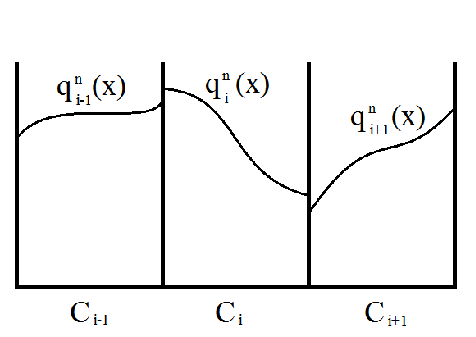
\includegraphics[angle=0,width=48mm]{FV/reconstruct.pdf} & 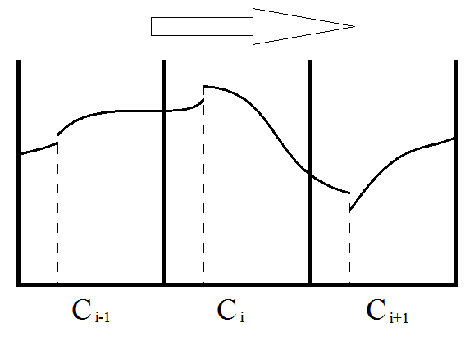
\includegraphics[angle=0,width=48mm]{FV/evolve.pdf} & 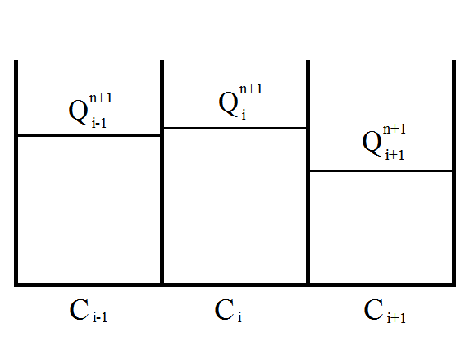
\includegraphics[angle=0,width=48mm]{FV/average.pdf}\\
{\small (1)} & {\small (2)} & {\small (3)}
\end{tabular}
\caption{REA algorithm with (1) Reconstruction phase, (2) evolution phase, and (3) cell averaging}
\end{figure}
\FloatBarrier
%%%%%%%%%%%%%%%%%%%%%%%%%%%%%%%%%%%%%%%%%%%%%%%%%%%%%%%%%%%%%%%%%%%%%%%%%%%%%%%
%%%%%%%%%%%%%%%%%%%%%%%%%%%%%%%%%%%%%%%%%%%%%%%%%%%%%%%%%%%%%%%%%%%%%%%%%%%%%%%
%%%%%%%%%%%%%%%%%%%%%%%%%%%%%%%%%%%%%%%%%%%%%%%%%%%%%%%%%%%%%%%%%%%%%%%%%%%%%%%
%%%%%%%%%%%%%%%%%%%%%%%%%%%%%%%%%%%%%%%%%%%%%%%%%%%%%%%%%%%%%%%%%%%%%%%%%%%%%%%
%%%%%%%%%%%%%%%%%%%%%%%%%%%%%%%%%%%%%%%%%%%%%%%%%%%%%%%%%%%%%%%%%%%%%%%%%%%%%%%
%%%%%%%%%%%%%%%%%%%%%%%%%%%%%%%%%%%%%%%%%%%%%%%%%%%%%%%%%%%%%%%%%%%%%%%%%%%%%%%
%%%%%%%%%%%%%%%%%%%%%%%%%%%%%%%%%%%%%%%%%%%%%%%%%%%%%%%%%%%%%%%%%%%%%%%%%%%%%%%
\subsection{CFL Condition For Stability}
A necessary condition for stability of FV methods, as well as FD methods, is the CFL condition. The CFL condition imposes a limit on the choice of the time step $\Delta t$ by the choice of the spatial step $\Delta x$. The CFL condition is defined by the relation
%
\begin{equation}
\label{CFLeq}
C = u \frac{\Delta t}{\Delta x}
\end{equation}
%
with some constraint on the constant $C$. This condition is attributed to Courant, Friedrich and Lewy \cite{cflCite}.

With the Godunov REA algorithm, the solutions in the cells will advect by some distance $u \Delta t$. See figure (\ref{CFLfig}). If this distance exceeds the cell length $\Delta x$, the cell values at the next time step will be influenced directly by cell values beyond the immediate neighboring cells. This effect is undesired because our methods depend on the flux from the neighboring cells. The resulting inequality is $u \Delta t \le \Delta x$. Rearranging terms and we obtain
%
\begin{equation*}
u \frac{\Delta t}{\Delta x} \le 1.
\end{equation*}
%
We find our constant to be $C = 1$ for the FV methods.
%Courant, Friedrich, and Lewy have shown that, by using finite difference methods they define a sequence of approximate solutions to certain PDE and shown that they converge and the limit must satisfy the PDE as the grid is refined. In LeVeque \cite{leveque} (pp. 69) The CFL condition is defined as: "A numerical method can be convergent only if its numerical domain of dependence contains the true domain of dependence of the PDE, at least in the limit as t and x go to zero." 
%
\begin{figure}[ht!]
  \centering
      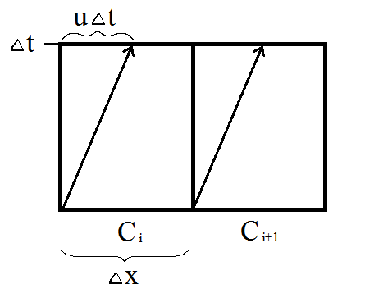
\includegraphics[angle=0,width=80mm]{CFL/cfl.pdf}
  \caption{after advection}
\label{CFLfig}
\end{figure}
\FloatBarrier
%
%The CFL condition is a necessary condition for both finite volume and finite difference methods for stability. For the transport equation, our gas advects from one cell to its neighbor after a time step of $\Delta t$ As can be seen in figure (\ref{CFLfig}). If the cell size $\Delta x$ is known, then the solution will advect a distance of $\Delta t u$. The finite volume methods we use will depend on neighboring cell values for the cell updates and so since $u$ is known the value of $\Delta t$ must be chosen such that $u \Delta t \le \Delta x$ or $u \Delta t = C \Delta x$ where $C <= 1$. Hence (\ref{CFLeq}).
%%%%%%%%%%%%%%%%%%%%%%%%%%%%%%%%%%%%%%%%%%%%%%%%%%%%%%%%%%%%%%%%%%%%%%%%%%%%%%%
%%%%%%%%%%%%%%%%%%%%%%%%%%%%%%%%%%%%%%%%%%%%%%%%%%%%%%%%%%%%%%%%%%%%%%%%%%%%%%%
%%%%%%%%%%%%%%%%%%%%%%%%%%%%%%%%%%%%%%%%%%%%%%%%%%%%%%%%%%%%%%%%%%%%%%%%%%%%%%%
%%%%%%%%%%%%%%%%%%%%%%%%%%%%%%%%%%%%%%%%%%%%%%%%%%%%%%%%%%%%%%%%%%%%%%%%%%%%%%%
%%%%%%%%%%%%%%%%%%%%%%%%%%%%%%%%%%%%%%%%%%%%%%%%%%%%%%%%%%%%%%%%%%%%%%%%%%%%%%%
%%%%%%%%%%%%%%%%%%%%%%%%%%%%%%%%%%%%%%%%%%%%%%%%%%%%%%%%%%%%%%%%%%%%%%%%%%%%%%%
%%%%%%%%%%%%%%%%%%%%%%%%%%%%%%%%%%%%%%%%%%%%%%%%%%%%%%%%%%%%%%%%%%%%%%%%%%%%%%%
%\section{First Order Approximation Method}
%In this section, we will derive the first order finite difference and finite volume methods and compare them. We will see that both methods are identical which will prove that the finite volume method we derive will be of first order accuracy.
%%%%%%%%%%%%%%%%%%%%%%%%%%%%%%%%%%%%%%%%%%%%%%%%%%%%%%%%%%%%%%%%%%%%%%%%%%%%%%%
%%%%%%%%%%%%%%%%%%%%%%%%%%%%%%%%%%%%%%%%%%%%%%%%%%%%%%%%%%%%%%%%%%%%%%%%%%%%%%%
%%%%%%%%%%%%%%%%%%%%%%%%%%%%%%%%%%%%%%%%%%%%%%%%%%%%%%%%%%%%%%%%%%%%%%%%%%%%%%%
%%%%%%%%%%%%%%%%%%%%%%%%%%%%%%%%%%%%%%%%%%%%%%%%%%%%%%%%%%%%%%%%%%%%%%%%%%%%%%%
\subsection{The First Order Finite Difference Method}
Let us derive the first order FD method for the transport equation. Recall the transport equation
%
\begin{equation}
\label{homoFirst}
\partial_t f(x,t) + u \partial_x f(x,t) = 0.
\end{equation}
%
A common practice for the derivation of FD methods stems from the Taylor series expansion. If $f$ is twice differentiable in time, then there exists $\xi_t \in [t,t+\Delta t]$ where
%
\begin{equation*}
f(x,t+\Delta t) = f(x,t) + \Delta t \partial_t f(x,t) + \frac{\Delta t^2}{2} \partial_t^2 f(x,\xi_t).
\end{equation*}
%
Writing the above equation in big O notation
%
\begin{equation*}
f(x,t+\Delta t) = f(x,t) + \Delta t \partial_t f(x,t) + O(\Delta t^2).
\end{equation*}
%
Similarly, if $f$ is twice differentiable in the $x$ variable, then we can approximate $f(x + \Delta x)$ by
%
\begin{equation*}
f(x + \Delta x,t) = f(x,t) + \Delta x \partial_x f(x,t) + O(\Delta x^2).
\end{equation*}
%
Notice that the dependence on the right nodal value ($x + \Delta x$) suggests we are solving for left moving waves $u<0$. Now from each of the expansions above, if we solve for $\partial_t f(x,t)$ and $\partial_x f(x,t)$ we obtain
%
\begin{align*}
&\partial_t f(x,t) = \frac{f(x,t+\Delta t) - f(x,t)}{\Delta t} + O(\Delta t)\\
&\partial_x f(x,t) = \frac{f(x+\Delta x,t) - f(x,t)}{\Delta x} + O(\Delta x)
\end{align*}
%
and substituting into (\ref{homoFirst}):
%
\begin{equation}
\label{dadada}
\left( \frac{f(x,t+\Delta t) - f(x,t)}{\Delta t} + O(\Delta t) \right) + u \left( \frac{f(x+\Delta x,t) - f(x,t)}{\Delta x} + O(\Delta x) \right) = 0.
\end{equation}
%
Solving for $f(x,t+\Delta t)$ from (\ref{dadada}):
%
\begin{equation*}
%\label{firstOrderHomo}
f(x,t+\Delta t) = f(x,t) - u \frac{\Delta t}{\Delta x} \left(f(x+\Delta x,t) - f(x,t)\right) + O(\Delta t^2) + O(\Delta x) \Delta t.
\end{equation*}
%
Recall from the CFL condition that $C \Delta x = u \Delta t$ and since $u$ is constant, $O(\Delta x) \Delta t = O(\Delta t^2)$ and so the above equation takes the form
%
\begin{equation}
\label{firstOrderHomoLeft}
f(x,t+\Delta t) = f(x,t) - u \frac{\Delta t}{\Delta x} \left(f(x+\Delta x,t) - f(x,t)\right) + O(\Delta t^2).
\end{equation}
%
The above equation is the first order FD method for solving (\ref{homoFirst}). Following the same process for right moving waves $u>0$, we obtain the equation using the left node ($x - \Delta x$)
%
\begin{equation}
\label{firstOrderHomoRight}
f(x,t+\Delta t) = f(x,t) - u \frac{\Delta t}{\Delta x} \left(f(x,t) - f(x - \Delta x,t)\right) + O(\Delta t^2).
\end{equation}
%%%%%%%%%%%%%%%%%%%%%%%%%%%%%%%%%%%%%%%%%%%%%%%%%%%%%%%%%%%%%%%%%%%%%%%%%%%%%%%
%%%%%%%%%%%%%%%%%%%%%%%%%%%%%%%%%%%%%%%%%%%%%%%%%%%%%%%%%%%%%%%%%%%%%%%%%%%%%%%
\subsection{The First Order Finite Volume Method}
We will now briefly derive the first order FV method. We start by employing Godunov's REA algorithm. Let $q_i^n(x) = Q_i^n$ be the constructed piecewise constant function approximating the solution at cell $C_i$ at time step $n$. During the time step the solutions are being transported to neighboring cells using the flux
%As we will see later, we can ignore the source term for now. We implement Godunov's method for linear systems by the reconstruct evolve average (REA) algorithm. This starts by reconstructing a polynomial approximation within a cell $C_i$ using the cell average, evolving the solution through time $\Delta t$, then developing the new cell average from which the process can be executed continuously over many time steps. For the first order approximation, Let's start with the assumption that our solution is piecewise constant in each cell. Given the velocity $u$ we can observe that the flux across the boundary through evolution will be given by
%
\begin{equation*}
\left\{
\begin{array}{cc}
F_{i-1/2}^n = u Q_{i-1}^n, & u>0\\
F_{i+1/2}^n = u Q_{i}^n, & u>0\\
F_{i-1/2}^n = u Q_{i}^n, & u<0\\
F_{i+1/2}^n = u Q_{i+1}^n, & u<0
\end{array}
\right.
\end{equation*}
%
where the direction of the flux depends on the sign of the velocity $u$. The new cell average is then determined as
%requires an addition from the incoming flux from the neighboring cell and subtracting off the flux lost to the other neighboring cell. So then evolving the solution at cell $C_i$ a time step $\Delta t$ later and averaging over the cell length $\Delta x$ our new cell averages become:
%
\begin{equation}
\label{first_order_FV_method}
\left\{
\begin{array}{cc}
Q_i^{n+1} = Q_i^n - u \frac{\Delta t}{\Delta x} (Q_{i}^n - Q_{i-1}^n), & u>0\\
Q_i^{n+1} = Q_i^n - u \frac{\Delta t}{\Delta x} (Q_{i+1}^n - Q_{i}^n), & u<0.
\end{array}
\right.
\end{equation}
%
Notice the above equations are the same as (\ref{firstOrderHomoLeft}) and (\ref{firstOrderHomoRight}) provided that the FD methods were derived using the function $f$ in the notation.
%Although the finite volume method is implemented for our use, we will observe that the first order finite difference approximation we obtain will yield the same result as the first order finite volume approach. This will also verify the first order accuracy of our FV method. This is not always the case as we will see later for a second order FV method.
%
%For the finite difference approximation consider the Taylor expansion of $f(x,t + \Delta t)$ through $t$ and $f(x + \Delta x,t)$ through $x$ for left moving waves:
%\begin{gather}
%\begin{aligned}
%\label{Taylor_expansion_1st_order}
%&f(x,t + \Delta t) = f(x,t) + \partial_t f(x,t) \Delta t + O(\Delta t^2)\\
%&f(x + \Delta x,t) = f(x,t) + \partial_x f(x,t) \Delta x + O(\Delta x^2)
%\end{aligned}
%\end{gather}
%
%Then the first derivative parts of each will be
%$$ \partial_x f(x,t) = \frac{f(x+\Delta x,t) - f(x,t)}{\Delta x} + O(\Delta x) $$
%$$ \partial_t f(x,t) = \frac{f(x,t+\Delta t) - f(x,t)}{\Delta t} + O(\Delta t) $$
%
%and by substituting this into (\ref{homoFirst}):
%$$ \left(\frac{f(x,t+\Delta t) - f(x,t)}{\Delta t} + O(\Delta t)\right) + \bar{u} \left(\frac{f(x+\Delta x,t) - f(x,t)}{\Delta x} + O(\Delta x)\right) = 0 $$ %\Psi (f(x,t))
%
%Then solving for $f(x,t+\Delta t)$:
%\begin{equation}
%f(x,t+\Delta t) = f(x,t) + \bar{u} \frac{\Delta t}{\Delta x} \left(f(x+\Delta x,t) - f(x,t)\right)% + \Delta t \Psi (f(x,t)) + O(\Delta t^2)
%\end{equation}
%
%Which is a first order accurate unsplit solution to $\ref{withSource}$. Note that by the CFL condition, a fixed $\Delta t$ is chosen so that $\Delta t = C \Delta x$ for some constant $C$ such that $0 < C \le \frac{1}{max(\bar{u_k}}$ then $O(\Delta x) = O(\Delta t)$. One can see the identical resemblance with \ref{first_order_FV_method}.
%%%%%%%%%%%%%%%%%%%%%%%%%%%%%%%%%%%%%%%%%%%%%%%%%%%%%%%%%%%%%%%%%%%%%%%%%%%%
%%%%%%%%%%%%%%%%%%%%%%%%%%%%%%%%%%%%%%%%%%%%%%%%%%%%%%%%%%%%%%%%%%%%%%%%%%%%
%%%%%%%%%%%%%%%%%%%%%%%%%%%%%%%%%%%%%%%%%%%%%%%%%%%%%%%%%%%%%%%%%%%%%%%%%%%%
%%%%%%%%%%%%%%%%%%%%%%%%%%%%%%%%%%%%%%%%%%%%%%%%%%%%%%%%%%%%%%%%%%%%%%%%%%%%
%%%%%%%%%%%%%%%%%%%%%%%%%%%%%%%%%%%%%%%%%%%%%%%%%%%%%%%%%%%%%%%%%%%%%%%%%%%%
%%%%%%%%%%%%%%%%%%%%%%%%%%%%%%%%%%%%%%%%%%%%%%%%%%%%%%%%%%%%%%%%%%%%%%%%%%%%
%%%%%%%%%%%%%%%%%%%%%%%%%%%%%%%%%%%%%%%%%%%%%%%%%%%%%%%%%%%%%%%%%%%%%%%%%%%%
%\section{Second Order Approximation Methods for the Advection Equation}
%In the first order advection method we assumed a piecewise constant solution for the advection problem and solved the source term using a first order forward Euler method. Similar to the first order method, our objective now is to develop a higher order method for the advection problem and for the source term. Because the fractional step method is only first order accurate, as shown before, our splitting method will employ Strang splitting. As long as the methods used for evolving the advection equation and the source term are both at least second order accurate then Strang splitting will guarantee that our combined solution will be at least second order accurate.
%%%%%%%%%%%%%%%%%%%%%%%%%%%%%%%%%%%%%%%%%%%%%%%%%%%%%%%%%%%%%%%%%%%%%%%%%%%%
%%%%%%%%%%%%%%%%%%%%%%%%%%%%%%%%%%%%%%%%%%%%%%%%%%%%%%%%%%%%%%%%%%%%%%%%%%%%
%%%%%%%%%%%%%%%%%%%%%%%%%%%%%%%%%%%%%%%%%%%%%%%%%%%%%%%%%%%%%%%%%%%%%%%%%%%%
%%%%%%%%%%%%%%%%%%%%%%%%%%%%%%%%%%%%%%%%%%%%%%%%%%%%%%%%%%%%%%%%%%%%%%%%%%%%
\subsection{The Second Order Finite Difference Method}
In this section, we will derive the second order FD method. The procedure is similar to the first order FD derivation except that second order terms are kept in the Taylor expansion. We start with the Taylor series expansion of $f(x,t+\Delta t)$ through time
%Since we observed that the first order FV method is identical to the first order FD method, it is only natural to question what makes the FV method different than the FD method. In this section we will derive the second order FD method and we will see that this is indeed a different result than the second order FV method. Then later we will show computed results showing that our FV method converges with second order accuracy.
%
\begin{equation*}
f(x,t+\Delta t) = f(x,t) + \Delta t \partial_t f(x,t) + \frac{\Delta t^2}{2} \partial_t^2 f(x,t) + O(\Delta t^3).
\end{equation*}
%
We want to derive a method to advance the solution a time step $\Delta t$. Because we don't have information about the solution through time but we do have information about the solution through $x$, we convert the time derivative terms in the above equation to the space derivative terms. By re-arranging (\ref{homoFirst}) in terms of $\partial_t f$
%
\begin{equation}
\label{firstPart}
\partial_t f = -u \partial_x f
\end{equation}
%
and also by the linearity of the differential operator
%
\begin{equation}
\label{secondPart}
\partial_t^2 f = \partial_t(\partial_t f) = \partial_t(-u \partial_x f) = -u \partial_x(\partial_t f) = -u \partial_x(-u \partial_x f) = u^2 \partial_x^2 f.
\end{equation}
%
%What we want to do here is since we are solving our system explicitly through time, we do not have information about the solution in the future time but we do have information about the solution through $x$ and so we can use (\ref{firstPart}) and (\ref{secondPart}) to replace the time derivatives of the Taylor expansion with the space derivative forms. This gives us
%
Using the above two relations, we replace the time derivative terms of the Taylor expansion by the spatial derivative terms
%
\begin{equation*}
f(x,t+\Delta t) = f(x,t) - u \Delta t \partial_x f(x,t) + u^2 \frac{\Delta t^2}{2} \partial_x^2 f(x,t) + O(\Delta t^3)
\end{equation*}
%
The central difference methods are then used to approximate the derivatives with second order accuracy:
%
\begin{align*}
f(x,t+\Delta t) =& f(x,t) - u \frac{\Delta t}{2 \Delta x} (f(x+\Delta x,t) - f(x-\Delta x,t))\\
&+ u^2 \frac{\Delta t^2}{2 \Delta x^2} (f(x-\Delta x,t) - 2 f(x,t) + f(x+\Delta x,t)) + O(\Delta t^3).
\end{align*}
%
The above is a second order accurate method to (\ref{homoFirst}). This is also known as the Lax–Wendroff method \cite{lax}.
%%%%%%%%%%%%%%%%%%%%%%%%%%%%%%%%%%%%%%%%%%%%%%%%%%%%%%%%%%%%%%%%%%%%%%%%%%%%
%%%%%%%%%%%%%%%%%%%%%%%%%%%%%%%%%%%%%%%%%%%%%%%%%%%%%%%%%%%%%%%%%%%%%%%%%%%%
%%%%%%%%%%%%%%%%%%%%%%%%%%%%%%%%%%%%%%%%%%%%%%%%%%%%%%%%%%%%%%%%%%%%%%%%%%%%
%%%%%%%%%%%%%%%%%%%%%%%%%%%%%%%%%%%%%%%%%%%%%%%%%%%%%%%%%%%%%%%%%%%%%%%%%%%%
\subsection{The Second Order Finite Volume Method}
We will derive the second order FV method for the transport equation using the same REA algorithm used for the first order FV method. The piecewise polynomial approximating the solution in cell $C_i$ at time $t_n$, in the first order FV method, used a constant polynomial equal to the cell average $Q_i$. In this section, we introduce a correction term to the piecewise polynomial by adding in a slope term $\sigma_i$. This slope is determined by an approximation to the derivative in $x$ by any conventional means. Let $q_i^n(x) = Q_i^n + \sigma_i (x - x_i)$ be the piecewise linear polynomial approximating the solution in cell $C_i$ at time $t_{n}$.
%Let us define $\mathring{q^n(x)}$ to be the exact solution at time step $n$ over the whole domain. We can better approximate the true solution everywhere in the domain if, in addition to the cell average at each cell, we approximate the slope of the solution. Let $Q_i$ refer to the cell average of at cell $C_i$ located at $x_i$. If we denote $\sigma_i$ to be the slope at cell $x_i$ then for all $x \in C_i$
%
%\begin{equation*}
%q_i^n(x) = Q_i^n + \sigma_i (x - x_i).
%\end{equation*}
%
%Notice that if our solution is smooth and if $q_i^n(x_i) = \mathring{q^n(x_i)}$ for each $i = 1,2,...,N$, then if our slope is approximated with at least second order accuracy then $q^n(x) - q_i^n(x) = O(\Delta x^2)$.
%
%There are two cases to look at. We can have advection to the right for positive moving waves $u>0$ or advection to the left for negative moving waves $u<0$. Since advection in one direction is the same process as in the other direction, we will observe positive velocities. referring to figure (), once we advect into cell $x_i$ the data is carried over by cell $Q_{i-1}$ ($Q_{i+1}$ if it's a left going wave). Note from figure (), if we advect to the right at some velocity $u$ then after some time $\Delta t$ the new cell average will be
%
%
%\begin{figure}[ht!]
%  \centering
%      \includegraphics[angle=0,width=140mm]{second_order/part1.jpg}
%  \caption{before advection}
%\label{before}
%\end{figure}
%%
%\begin{figure}[ht!]
%  \centering
%      \includegraphics[angle=0,width=140mm]{second_order/part2.jpg}
%  \caption{after advection}
%\label{after}
%\end{figure}
%\FloatBarrier
%
Let's derive the flux at the left boundary due to positive moving waves. Because we have a piecewise linear approximation at the left cell, the flux entering the cell from the left, $C_{i-1}$, is
%
\begin{align*}
%\label{FluxBoundaryLeft}
F_{i-1/2}^n &= \frac{1}{\Delta t} \int_{x_{i-1} + \frac{\Delta x}{2} - u \Delta t}^{x_{i-1} + \frac{\Delta x}{2}} q_{i-1}^n(x) dx \nonumber\\
&= \frac{1}{\Delta t} \int_{x_{i-1} + \frac{\Delta x}{2} - u \Delta t}^{x_{i-1} + \frac{\Delta x}{2}} Q_{i-1}^n + \sigma_{i-1}^n (x-x_{i-1}) dx \nonumber \\
&= \left( Q_{i-1}^n + \frac{\sigma_{i-1}^n}{2} (\Delta x - u \Delta t) \right) u
\end{align*}
%
and computing the flux leaving the cell $C_i$ at the right boundary is
%
\begin{align*}
%\label{FluxBoundaryRight}
F_{i+1/2}^n &= \frac{1}{\Delta t} \int_{x_i + \frac{\Delta x}{2} - u \Delta t}^{x_i + \frac{\Delta x}{2}} q_i^n(x) dx \nonumber\\
&= \frac{1}{\Delta t} \int_{x_i + \frac{\Delta x}{2} - u \Delta t}^{x_i + \frac{\Delta x}{2}} Q_i^n + \sigma_i^n (x-x_i) dx \nonumber\\
&= \left( Q_i^n + \frac{\sigma_{i}^n}{2} (\Delta x - u \Delta t) \right) u.
\end{align*}
%
Performing the same procedure to find the fluxes for left moving waves ($u<0$) and combining with the fluxes derived above provides the resulting fluxes
%
\begin{equation*}
\left\{
\begin{array}{cc}
F_{i-1/2}^n = \left( Q_{i-1}^n + \frac{\sigma_{i-1}^n}{2} (\Delta x - u \Delta t) \right) u, & u>0\\
F_{i+1/2}^n = \left( Q_i^n + \frac{\sigma_{i}^n}{2} (\Delta x - u \Delta t) \right) u, & u>0\\
F_{i-1/2}^n = \left( Q_{i}^n - \frac{\sigma_{i}^n}{2} (\Delta x + u \Delta t) \right) u, & u<0\\
F_{i+1/2}^n = \left( Q_{i+1}^n - \frac{\sigma_{i+1}^n}{2} (\Delta x + u \Delta t) \right) u, & u<0.
\end{array}
\right.
\end{equation*}
%
The new cell averages are obtained by implementing the above flux terms into (\ref{FVmethod})
%
\begin{equation}
\label{secondOrdFV}
\left\{
\begin{array}{cc}
Q_i^{n+1} = Q_i^n - \frac{u \Delta t}{\Delta x} (Q_i^n - Q_{i-1}^n) - \frac{1}{2} \frac{u \Delta t}{\Delta x} (\Delta x - u \Delta t) (\sigma_i^n - \sigma_{i-1}^n), \, & u > 0\\
Q_i^{n+1} = Q_i^n - \frac{u \Delta t}{\Delta x} (Q_{i+1}^n - Q_i^n) + \frac{1}{2} \frac{u \Delta t}{\Delta x} (\Delta x + u \Delta t) (\sigma_{i+1}^n - \sigma_i^n), \, & u < 0.
\end{array}
\right.
\end{equation}
%
%To find the solution at an arbitrary point $x \in X_i$ we make use of the slope $\sigma_i$ and the cell average which is also the center value $Q_i$ at time step $n$ we have:
%
%\begin{equation}
%\label{Qin}
%Q_i^n(x) = \sigma_i^n (x - x_{i-1})
%\end{equation}
%To get area 1 after advecting to the right, the right end point is $Q_{i-1}^n(x_{i-1}^n + \frac{\Delta x}{2})$ and the value at the left of area 1 is $Q_{i-1}^n(x_{i-1}+\frac{\Delta x}{2}-u \Delta t)$ and applying the same concept to get area 2 where we want to keep what is left of the cell and not has left. At the end, we arrive at the results of areas 1 and 2:
%\begin{equation}
%\label{Area1}
%A_1 = \frac{1}{2} (Q_{i-1}^n + \sigma_{i-1}^n (\frac{1}{2} \Delta x) + Q_{i-1}^n + \sigma_{i-1}^n (\frac{1}{2} \Delta %x - u \Delta t)) u \Delta t
%\end{equation}
%\begin{equation}
%\label{Area2}
%A_2 = \frac{1}{2} (Q_{i}^n + \sigma_i^n (-\frac{1}{2} \Delta x) + Q_{i-1}^n + \sigma_{i}^n (\frac{1}{2} \Delta x - u %\Delta t)) (\Delta x - u \Delta t)
%\end{equation}
%Then, the result final solution at cell $X_i$ at time step $n+1$ is
%$$ Q_i^{n+1} = (A_1 + A_2) \frac{1}{\Delta x} $$
%which comes out to be
%
%Then combining (\ref{FluxBoundaryLeft}) and (\ref{FluxBoundaryRight}) into (\ref{FVmethod}) we get
%\begin{equation}
%\label{Right}
%Q_i^{n+1} = Q_i^n - \frac{u \Delta t}{\Delta x} (Q_i^n - Q_{i-1}^n) - \frac{1}{2} \frac{u \Delta t}{\Delta x} (\Delta x - u \Delta t) (\sigma_i^n - \sigma_{i-1}^n), \, u > 0.
%\end{equation}
%
%Applying the same procedure for left moving waves we get
%
%\begin{equation}
%\label{Left}
%Q_i^{n+1} = Q_i^n - \frac{u \Delta t}{\Delta x} (Q_{i+1}^n - Q_i^n) + \frac{1}{2} \frac{u \Delta t}{\Delta x} (\Delta x + u \Delta t) (\sigma_{i+1}^n - \sigma_i^n), \, u < 0.
%\end{equation}
%
% R.LeVeques equation (6.13) on page 107
%Note that we have conserved the flux across the boundary yet we have introduced an additional correction term to our flux. Also,

The choice of the slope has no effect on the conservation of the method but if we let $\sigma = 0$ we will get the first order method back. The choice of the slope depends on the approximation of the derivative. For our case, we use the center difference slope which has an accuracy of $O(\Delta x^2)$
%
\begin{equation*}
%\label{CenterDiff}
\sigma_i^n = \frac{Q_{i+1}^n-Q_{i-1}^n}{2 \Delta x}.
\end{equation*}
%
Notice that the second order FV methods (\ref{secondOrdFV}) are not the same as the second order FD methods obtained earlier.
%%%%%%%%%%%%%%%%%%%%%%%%%%%%%%%%%%%%%%%%%%%%%%%%%%%%%%%%%%%%%%%%%%%%%%%%%
%To handle the right hand side, we split the problem into two parts. The first part is the homogeneous form of our PDE that we solve over one time step. Then the second part is of the form $q_t = B q$ which we solve for a half time step. The method we use starts by solving the B problem (as in R. LeVeques book) over a half time step then the A problem with a full time step then the B problem again with a half time step. (page 387 explains why this preserves higher order accuracy) which is known as Strang Splitting. Since we do not have information about the derivative, we can get second order accuracy with the second order Runge Kutta method for the B step.
%%%%%%%%%%%%%%%%%%%%%%%%%%%%%%%%%%%%%%%%%%%%%%%%%%%%%%%%%%%%%%%%%%%%%%%%%%%%%%%
%%%%%%%%%%%%%%%%%%%%%%%%%%%%%%%%%%%%%%%%%%%%%%%%%%%%%%%%%%%%%%%%%%%%%%%%%%%%%%%
\subsection{Two Step Runge Kutta for the Collision Operator of the Kinetic Models}
The use of a splitting method described in the next section, the solution to the model kinetic equation can be done by advancing the transport and the collision part of the equations in alternating fashion. Thus in the first step one solves the transport equation using either the first or second order techniques. In the second step, the collision part of the model equation if solved in one temporal interval.
%
\begin{equation}
\label{2271}
\partial_t f(x,t) = \Psi(f).
\end{equation}
%
In case when analytical solution is not available and the equation needs to be solved numerically, the order of accuracy for the time integration has to be consistent with the desired order of the splitting technique. In particular, if the first order splitting technique is sought, then the scheme advancing (\ref{2271}) in time should be first order and if second order splitting is desired, then second order time integration should be used to advance solution to (\ref{2271}) in time. In the case of the first order splitting, one can use Euler's method to discretize (\ref{2271}) in time. In the case of second order splitting, a second order time discretization scheme needs to be proposed. In this approach we do not have the convenience of trading derivatives used in the derivation of second order method (\ref{firstPart})-(\ref{secondPart}). Instead, to achieve second order accuracy we apply a two-stage Runge-Kutta method. Namely,
%
\begin{align*}
k_1 &= Q_i + \frac{\Delta t}{2} \Psi(f,t_n)\\
Q_i^{n+1} &= Q_i^n + \Delta t \Psi(k_1,t_n + \Delta t/2).
\end{align*}
%%%%%%%%%%%%%%%%%%%%%%%%%%%%%%%%%%%%%%%%%%%%%%%%%%%%%%%%%%%%%%%%%%%%%%%%%%%%
%%%%%%%%%%%%%%%%%%%%%%%%%%%%%%%%%%%%%%%%%%%%%%%%%%%%%%%%%%%%%%%%%%%%%%%%%%%%
%%%%%%%%%%%%%%%%%%%%%%%%%%%%%%%%%%%%%%%%%%%%%%%%%%%%%%%%%%%%%%%%%%%%%%%%%%%%
%%%%%%%%%%%%%%%%%%%%%%%%%%%%%%%%%%%%%%%%%%%%%%%%%%%%%%%%%%%%%%%%%%%%%%%%%%%%
%%%%%%%%%%%%%%%%%%%%%%%%%%%%%%%%%%%%%%%%%%%%%%%%%%%%%%%%%%%%%%%%%%%%%%%%%%%%
%%%%%%%%%%%%%%%%%%%%%%%%%%%%%%%%%%%%%%%%%%%%%%%%%%%%%%%%%%%%%%%%%%%%%%%%%%%%
%%%%%%%%%%%%%%%%%%%%%%%%%%%%%%%%%%%%%%%%%%%%%%%%%%%%%%%%%%%%%%%%%%%%%%%%%%%%
\section{Splitting Methods}
In this section we discuss the splitting methods for splitting the BGK and ES-BGK kinetic models of the form
%
\begin{equation}
\label{kineticModel}
\partial_t f + u \, \partial_x f = \Psi (f).
\end{equation}
%
Obviously, the FV methods discussed will not solve the above equation directly. Instead, the FV methods solve the homogeneous transport equation
%
\begin{equation}
\label{homo}
\partial_t f + u \partial_x f = 0.
\end{equation}
%
To include the source term, we make use of the solution to the ODE describing $f$ along the characteristic curve of (\ref{kineticModel}) namely
%
\begin{equation}
\label{char}
\frac{df}{dt} = \Psi (f).
\end{equation}
%
Along the characteristic ($dx/dt = u$), the homogeneous equation remains constant through time. For this reason, we advance the solution to (\ref{kineticModel}) through time by advancing the transport equation through time then update the solution by advancing (\ref{char}). This is the idea behind the splitting methods.
%In many cases, solving the kinetic equations directly may be more difficult than if we were to solve the homogeneous form first then solve along the characteristic which can be expressed as a simple ODE. Here we will derive splitting methods that will allow us to solve for $f$ with first order accuracy and for higher accuracy.
%%%%%%%%%%%%%%%%%%%%%%%%%%%%%%%%%%%%%%%%%%%%%%%%%%%%%%%%%%%%%%%%%%%%%%%%%%%%
%%%%%%%%%%%%%%%%%%%%%%%%%%%%%%%%%%%%%%%%%%%%%%%%%%%%%%%%%%%%%%%%%%%%%%%%%%%%
%%%%%%%%%%%%%%%%%%%%%%%%%%%%%%%%%%%%%%%%%%%%%%%%%%%%%%%%%%%%%%%%%%%%%%%%%%%%
\subsection{Fractional Step Method}
The fractional step method allows us to perform first order splitting of (\ref{kineticModel}).
%leveque - why this is only first order accurate
%R. LeVeque page 380
In R. LeVeque \cite{leveque}, it is claimed that if we solve for (\ref{homo}) with first order accuracy over a whole time step $\Delta t$ then use that intermediate value to advance (\ref{char}) over a whole time step with first order accuracy, then we will have solved (\ref{kineticModel}) over a whole time step with first order accuracy in both $x$ and $t$. We will briefly verify this claim. Consider the unsplit form (\ref{kineticModel}). Let us update our solution over a time step of $\Delta t$ for left going waves $u<0$ (right going waves follow the same procedure) by
%
\begin{equation}
\label{firstOrderUnsplit}
f(x,t+\Delta t) = f(x,t) + \bar{u} \frac{\Delta t}{\Delta x} \left(f(x+\Delta x,t) - f(x,t)\right) + \Delta t \Psi(f(x,t)) + O(\Delta t^2).
\end{equation}
%

Now, consider that we update our solution by first advancing (\ref{homo}) by a time step $\Delta t$ from the above equation and call it $f^*(x,t)$. Then use the forward Euler approximation of the time evolution of (\ref{char}). We would then have a two step form process of the numerical solution as follows
%
\begin{align*}
\text{step A}& \quad f^*(x,t) = \left\{ \begin{array}{cl} f(x,t) + u \frac{\Delta t}{\Delta x} \left(f(x+\Delta x,t) - f(x,t)\right) & u<0\\
f(x,t) + u \frac{\Delta t}{\Delta x} \left(f(x,t) - f(x - \Delta x,t)\right) & u>0 \end{array} \right.\\
\text{step B}& \quad f(x,t+\Delta t) = f^*(x,t) + \Delta t \Psi(f^*(x,t)).
\end{align*}
%
We can see that by substituting the result from Step A directly into step B we get something similar to the unsplit method with the only difference being that the $\Psi(f(x,t))$ term in the unsplit method is replaced by the $\Psi(f^*(x,t))$ term. We can see from (\ref{firstOrderUnsplit}) that $f^*(x,t) = f(x,t) + O(\Delta t)$ and so
%
\begin{align*}
\Psi(f^*(x,t)) &= \Psi \left(f(x,t) + O(\Delta t) \right)\\
&= \Psi \left(f(x,t) \right) + O(\Delta t)
\end{align*}
%
giving us the expanded form (for left moving waves $u<0$)
%
\begin{equation*}
f(x,t+\Delta t) = f(x,t) + \bar{u} \frac{\Delta t}{\Delta x} \left(f(x+\Delta x,t) - f(x,t)\right) + \Delta t \Psi(f(x,t)) + O(\Delta t^2)
\end{equation*}
%
We notice that the form of this expression agrees with the unsplit method at the same level of accuracy. It may appear as if we have advanced the solution by two time steps, but we have advected the solution then updated the solution from the source term. This splitting technique is limited to first order approximation and a different technique for higher order accuracy will be looked at next.
%%%%%%%%%%%%%%%%%%%%%%%%%%%%%%%%%%%%%%%%%%%%%%%%%%%%%%%%%%%%%%%%%%%%%%%%%%%%%%%
%%%%%%%%%%%%%%%%%%%%%%%%%%%%%%%%%%%%%%%%%%%%%%%%%%%%%%%%%%%%%%%%%%%%%%%%%%%%%%%
%%%%%%%%%%%%%%%%%%%%%%%%%%%%%%%%%%%%%%%%%%%%%%%%%%%%%%%%%%%%%%%%%%%%%%%%%%%%%%%
%%%%%%%%%%%%%%%%%%%%%%%%%%%%%%%%%%%%%%%%%%%%%%%%%%%%%%%%%%%%%%%%%%%%%%%%%%%%%%%
%%%%%%%%%%%%%%%%%%%%%%%%%%%%%%%%%%%%%%%%%%%%%%%%%%%%%%%%%%%%%%%%%%%%%%%%%%%%%%%
%%%%%%%%%%%%%%%%%%%%%%%%%%%%%%%%%%%%%%%%%%%%%%%%%%%%%%%%%%%%%%%%%%%%%%%%%%%%%%%
%%%%%%%%%%%%%%%%%%%%%%%%%%%%%%%%%%%%%%%%%%%%%%%%%%%%%%%%%%%%%%%%%%%%%%%%%%%%%%%
\subsection{Linear Strang Splitting}
The fractional step method will give first order accuracy as long as (\ref{homo}) and (\ref{char}) are first order accurate. Unfortunately, it will not provide second order or above accuracy no matter how accurate the methods used in the solution of Step A and Step B are. To compensate for this, Strang splitting is introduced where the solution can be computed over different sized time steps. In Strang \cite{strang} linear equations with operators $A$ and $B$ of the form
%
\begin{equation}
\label{linearEq}
\partial_t f = A f + B f
\end{equation}
%
have the exact solution of the form
%
\begin{equation}
f(x,t_0 + \Delta t) = e^{\Delta t (A + B)}f(x,t_0).
\end{equation}
%
Rather than solving (\ref{linearEq}) directly, one solves the equations
%
\begin{equation}
\label{partA}
\partial_t f = A f
\end{equation}
%
and
%
\begin{equation}
\label{partB}
\partial_t f = B f
\end{equation}
%
while keeping the solution $f$ updated in time in the order they are evaluated. In the case that the operators $A$ and $B$ are commutable, this is as simple as solving (\ref{partA}) with a whole time step. Indeed, in this case, $f(x,t_0 + \Delta t) = e^{\Delta t A}e^{\Delta t B} f(x,t_0) = e^{\Delta t (A + B)} f(x,t_0)$. However, in general, operators $A$ and $B$ do not commute. Strang (1968) \cite{strang} has proposed to solve (\ref{partA}) over a half time step. Use the result in (\ref{partB}) over a whole time step. Then use that result in (\ref{partA}) again over a half time step. The result will be second order accurate provided that each of the steps are at least second order accurate. The combined result of the three steps can be written as
%
\begin{equation}
\label{Strang2}
f(x,t_0+\Delta t) \approx e^{\frac{\Delta t}{2} A} e^{\Delta t B} e^{\frac{\Delta t}{2} A} f(x,t_0).
\end{equation}
%
\begin{figure}[h!]
  \centering
      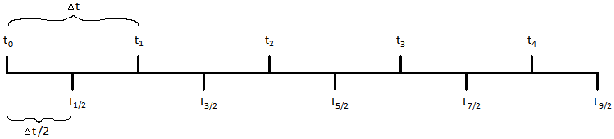
\includegraphics[angle=0,width=150mm]{strang/strang.pdf}
  \caption{\label{strang_interval} The top marks illustrate the time steps for the fractional step method. The bottom marks illustrate the time steps for the Strang splitting. The solution to the kinetic model equation is advanced a whole time step at every $t_{2n}$ for $n=1,2,3,...$.}
\end{figure}
\FloatBarrier
%
Expanding out each of the exponents of the RHS of (\ref{Strang2}) through Taylor series and multiplying together we get
%
\begin{align*}
e^{\frac{\Delta t}{2} A} e^{\Delta t B} e^{\frac{\Delta t}{2} A} &= 1 + \Delta t \left(\frac{1}{2} A + B + \frac{1}{2} A\right)\\
&+ \Delta t^2 \left(\frac{1}{8} A^2 + \frac{1}{2} A B + \frac{1}{2} B^2 + \frac{1}{4} A^2 + \frac{1}{2} B A + \frac{1}{8} B^2 \right) + O(\Delta t^3)\\
&= 1 + \Delta t (A + B) + \frac{\Delta t^2}{2}(A + B)^2 + O(\Delta t^3).
\end{align*}
%
Preserving the second order accuracy of the method.
%%%%%%%%%%%%%%%%%%%%%%%%%%%%%%%%%%%%%%%%%%%%%%%%%%%%%%%%%%%%%%%%%%%%%%%%%%%%%%%
%%%%%%%%%%%%%%%%%%%%%%%%%%%%%%%%%%%%%%%%%%%%%%%%%%%%%%%%%%%%%%%%%%%%%%%%%%%%%%%
%%%%%%%%%%%%%%%%%%%%%%%%%%%%%%%%%%%%%%%%%%%%%%%%%%%%%%%%%%%%%%%%%%%%%%%%%%%%%%%
%%%%%%%%%%%%%%%%%%%%%%%%%%%%%%%%%%%%%%%%%%%%%%%%%%%%%%%%%%%%%%%%%%%%%%%%%%%%%%%
%%%%%%%%%%%%%%%%%%%%%%%%%%%%%%%%%%%%%%%%%%%%%%%%%%%%%%%%%%%%%%%%%%%%%%%%%%%%%%%
%%%%%%%%%%%%%%%%%%%%%%%%%%%%%%%%%%%%%%%%%%%%%%%%%%%%%%%%%%%%%%%%%%%%%%%%%%%%%%%
\subsection{Non-Linear Strang Splitting}
In many applications where high resolution methods are desired for linear equations, Strang splitting is guaranteed to work. Here, we will show that Strang splitting will still give us second order accuracy for nonlinear systems of equations given that each step is at least second order accurate. Jianke Yang \cite{yang} (page 336-340) has shown that nonlinear Strang splitting methods will work up to fourth order accuracy. This is important to consider since in the case of the kinetic models used, the right hand side of the BGK and ES-BGK equations are a nonlinear operators. The set up for the nonlinear methods will be the same as with the linear methods. Consider ($\ref{linearEq}$) but now replace the linear operators $A$ and $B$ with the non-linear operators $M$ and $N$ so that the general equation is of the form of
\begin{equation}
\label{nonLinearEq}
\partial_t f = M(f) + N(f).
\end{equation}
%
We will split ($\ref{nonLinearEq}$) into two parts to be integrated separately, namely
\begin{equation}
\label{part1}
\partial_t f = M(f)
\end{equation}
%
and
\begin{equation}
\label{part2}
\partial_t f = N(f).
\end{equation}
%
The idea here is to evaluate the integral of the first equation (\ref{part1}) over a half time step. Use that result to then advance the solution in the second equation (\ref{part2}) over a whole time step. Then use this result again in a half time step evolution in the first equation. By repeating this process we can see that the last step is evaluated again over a half time step and so we can evaluate both components over a whole time step but offset by $\frac{\Delta t}{2}$ suggesting a similarity to the fractional step method. Because of the symmetric structure of (\ref{nonLinearEq}) we choose  to associate with the first step does not matter. However, to be specific, let us first start with (\ref{part1}). Just like with the linear Strang splitting, we will proceed to integrate ($\ref{part1}$) over a half time step $\frac{\Delta t}{2}$ from $t_0$ and designate this result with $f^*$
%
\begin{equation}
\label{v1}
f^* = f(x,t_0) + M(f(x,t_0)) \frac{\Delta t}{2} + \nabla M(M(f(x,t_0))) \frac{\Delta t^2}{8} + O(\Delta t^3).
\end{equation}
%
We then integrate ($\ref{part2}$) over a whole time step $\Delta t$ starting at $f^*$ and designate the next result with $f^{**}$.
%
\begin{equation}
\label{v2}
f^{**} = f^* + N(f^*) \Delta t + \frac{\Delta t^2}{2} \nabla N(N(f^*)) + O(\Delta t^3).
\end{equation}
%
Notice that
%
\begin{equation}
\label{Nv1}
N(f^*) = N \left(u_0 + \frac{1}{2} M \Delta t + O(\Delta t^2)\right) = N(f_0) + \frac{1}{2} \nabla N(M(f_0)) \Delta t + O(\Delta t^2)
\end{equation}
%
and
%
\begin{equation}
\label{NNv1}
\nabla N\left(N(f^*)\right) = \nabla N \left(N(f_0) + \frac{1}{2} \nabla N(M(f_0)) \Delta t + O(\Delta t^2) \right) = \nabla N\left(N(f_0)\right) + O(\Delta t)
\end{equation}
%
we substitute (\ref{v1}) into (\ref{v2}) and expand the result to the form
%
\begin{equation}
f^{**} = f_0 + \left(\frac{1}{2} M + N \right) \Delta t + \frac{1}{2} \left[ \frac{1}{4} \nabla M\left(M \right) + \nabla N\left(M+N \right)\right] \Delta t^2 + O(\Delta t^3).
\end{equation}
%
At the final step, we evaluate ($\ref{part1}$) over a half time step $\frac{\Delta t}{2}$ starting from our latest solution $f^{**}$ to get
%
\begin{equation}
\label{fss}
f(x,t_0+\Delta t) = f^{**} + \frac{1}{2} M(f^{**}) \Delta t + \frac{1}{8} \nabla M \left( M(f^{**}) \right) \Delta t^2 + O(\Delta t^3).
\end{equation}
%
If we expand the $M(f^{**})$ term we see that
%
\begin{equation}
\label{Mfss}
M(f^{**}) = M\left(f_0 + \left(\frac{1}{2}M + N \right) \Delta t + O(\Delta t^2)\right) = M + \nabla M(\frac{1}{2} M + N) \Delta t + O(\Delta t^2)
\end{equation}
%
and so
%
\begin{equation}
\label{MMfss}
\nabla M \left(M(f^{**})\right) = \nabla M\left(M + O(\Delta t)\right) = \nabla M\left(M \right) + O(\Delta t).
\end{equation}
%
Substituting (\ref{Mfss}) and (\ref{MMfss}) into (\ref{fss}) we get
%
\begin{equation*}
f(x,t+\Delta t) = f_0 + \left(\frac{1}{2} M + N \right) \Delta t + \frac{1}{2} \left[ \frac{1}{4} \nabla M \left(M \right) + \nabla N\left (M + N \right) \right] \Delta t^2
\end{equation*}
\begin{equation*}
 + \frac{1}{2} \left[M + \nabla M(\frac{1}{2} M + N) \Delta t \right] \Delta t + \frac{1}{8} \nabla M(M) \Delta t^2 + O(\Delta t^3).
\end{equation*}
%
After simplification,
%
\begin{equation}
f(x,t+\Delta t) = f_0 + \left(M + N\right) \Delta t + \frac{1}{2} \left[ \nabla (M + N)(M + N) \right] \Delta t^2 + O(\Delta t^3).
\end{equation}
%
%Now, $N(v_1) = N(u_0 + \zeta) = N(u_0) + N_t (u_0) \zeta + O(\zeta^2)$ where $\zeta = M(u_0) \frac{h}{2} + M_t(u_0) \frac{h^2}{8} + O(h^3)$ and consequently $O(\zeta) = O(h)$ So then
%
%$$ N(v_1) = N(u_0) + N_t(u_0) \left(M(u_0) \frac{h}{2} + M_t(u_0) \frac{h^2}{8}\right) + O(h^3) $$
%
%$$ N(v_1) = N(u_0) + N_t(u_0) M(u_0) \frac{h}{2} + N_t(u_0) M_t(u_0) \frac{h^2}{8} + O(h^3) $$
%
%$$ N_t (v_1) = N(u_0) + O(h) $$
%then substituting into the $v_2$ equation
%
%$$
%v_2 = v_1 + N(u_0) h + N_t(u_0) M(u_0) \frac{h^2}{2} + N_t(u_0) M_t(u_0) \frac{h^3}{8} + \frac{h^2}{2} N_t (v_1) + O(h^3)
%$$
%%%%%%%%%%%%%%%%%%%%%%%%%%%%%%%%%%%%%%%%%%%%%%%%%%%%%%%%%%%%%%%%%%%%%%%%%%%%%%%
This is a general formulation for nonlinear equations. For our implementation, we will have $M(f) = \nu (f_0 - f)$, the relaxation term, and $N(f) = -\partial_x f$, the differential operator through $x$ operated on f. For our system the $N(f)$ term is linear but the $M(f)$ term is nonlinear. We implement Strang splitting for the second order solver in the CLAWPACK software package.
